% !TeX root = ..\protokoll.tex
\documentclass[../protokoll.tex]{subfiles}
\graphicspath{{\subfix{../images/}}}
\begin{document}
\section{Abschwächung von \texorpdfstring{$\gamma$}{Gamma}-Strahlung in Materie}\label{sec:Abschwächung Gamma-Strahlung}
In diesem Versuch wird die Abschwächung der $\gamma$-Strahlung durch Eisenplatten verschiedener Dicken gemessen. Der Aufbau entspricht dem aus den vorangegangenen Messungen. Es wird das Sr-90-Präparat in dem Abstand $d_1$=100 mm vom Detektor aufgebaut, während die Eisenplatten jeweils in einem Abstand von 50 mm aufgebaut werden. Die Dicke x der Platten wird dabei variiert. Die Messzeit $\Delta t$ beträgt jeweils 60 s. Es wird die Nettozählrate n ermittelt, indem die Messrate m aus der gemessenen Impulszahl M bestimmt wird und dann die vorher bestimmte Nulleffekt-Zählrate $m_0$ abgezogen wird.
\begin{equation}
        n=m-m_0
\end{equation}
Die Messwerte sind in \ref{tab3} dargestellt.
\begin{table}[h]
\centering
\begin{tabular}{|l|l|l|}
\hline
x in mm & M     & n in 1/s \\ \hline
5       & 17802 & 296,7    \\ \hline
10      & 14839 & 247,32   \\ \hline
15      & 12585 & 209,75   \\ \hline
20      & 10678 & 177,97   \\ \hline
25      & 9117  & 151,95   \\ \hline
30      & 7784  & 129,73   \\ \hline
35      & 6768  & 112,8    \\ \hline
40      & 5952  & 99,1     \\ \hline
\end{tabular}
\caption{Gemessene Impulszahl M und ausgerechnete Nettozählrate n in Abhängigkeit der Dicke x}
\label{tab3}
\end{table}
Die Werte von n sind über x in \ref{beta1} halblogarithmisch aufgetragen.
\begin{figure}
    \centering
    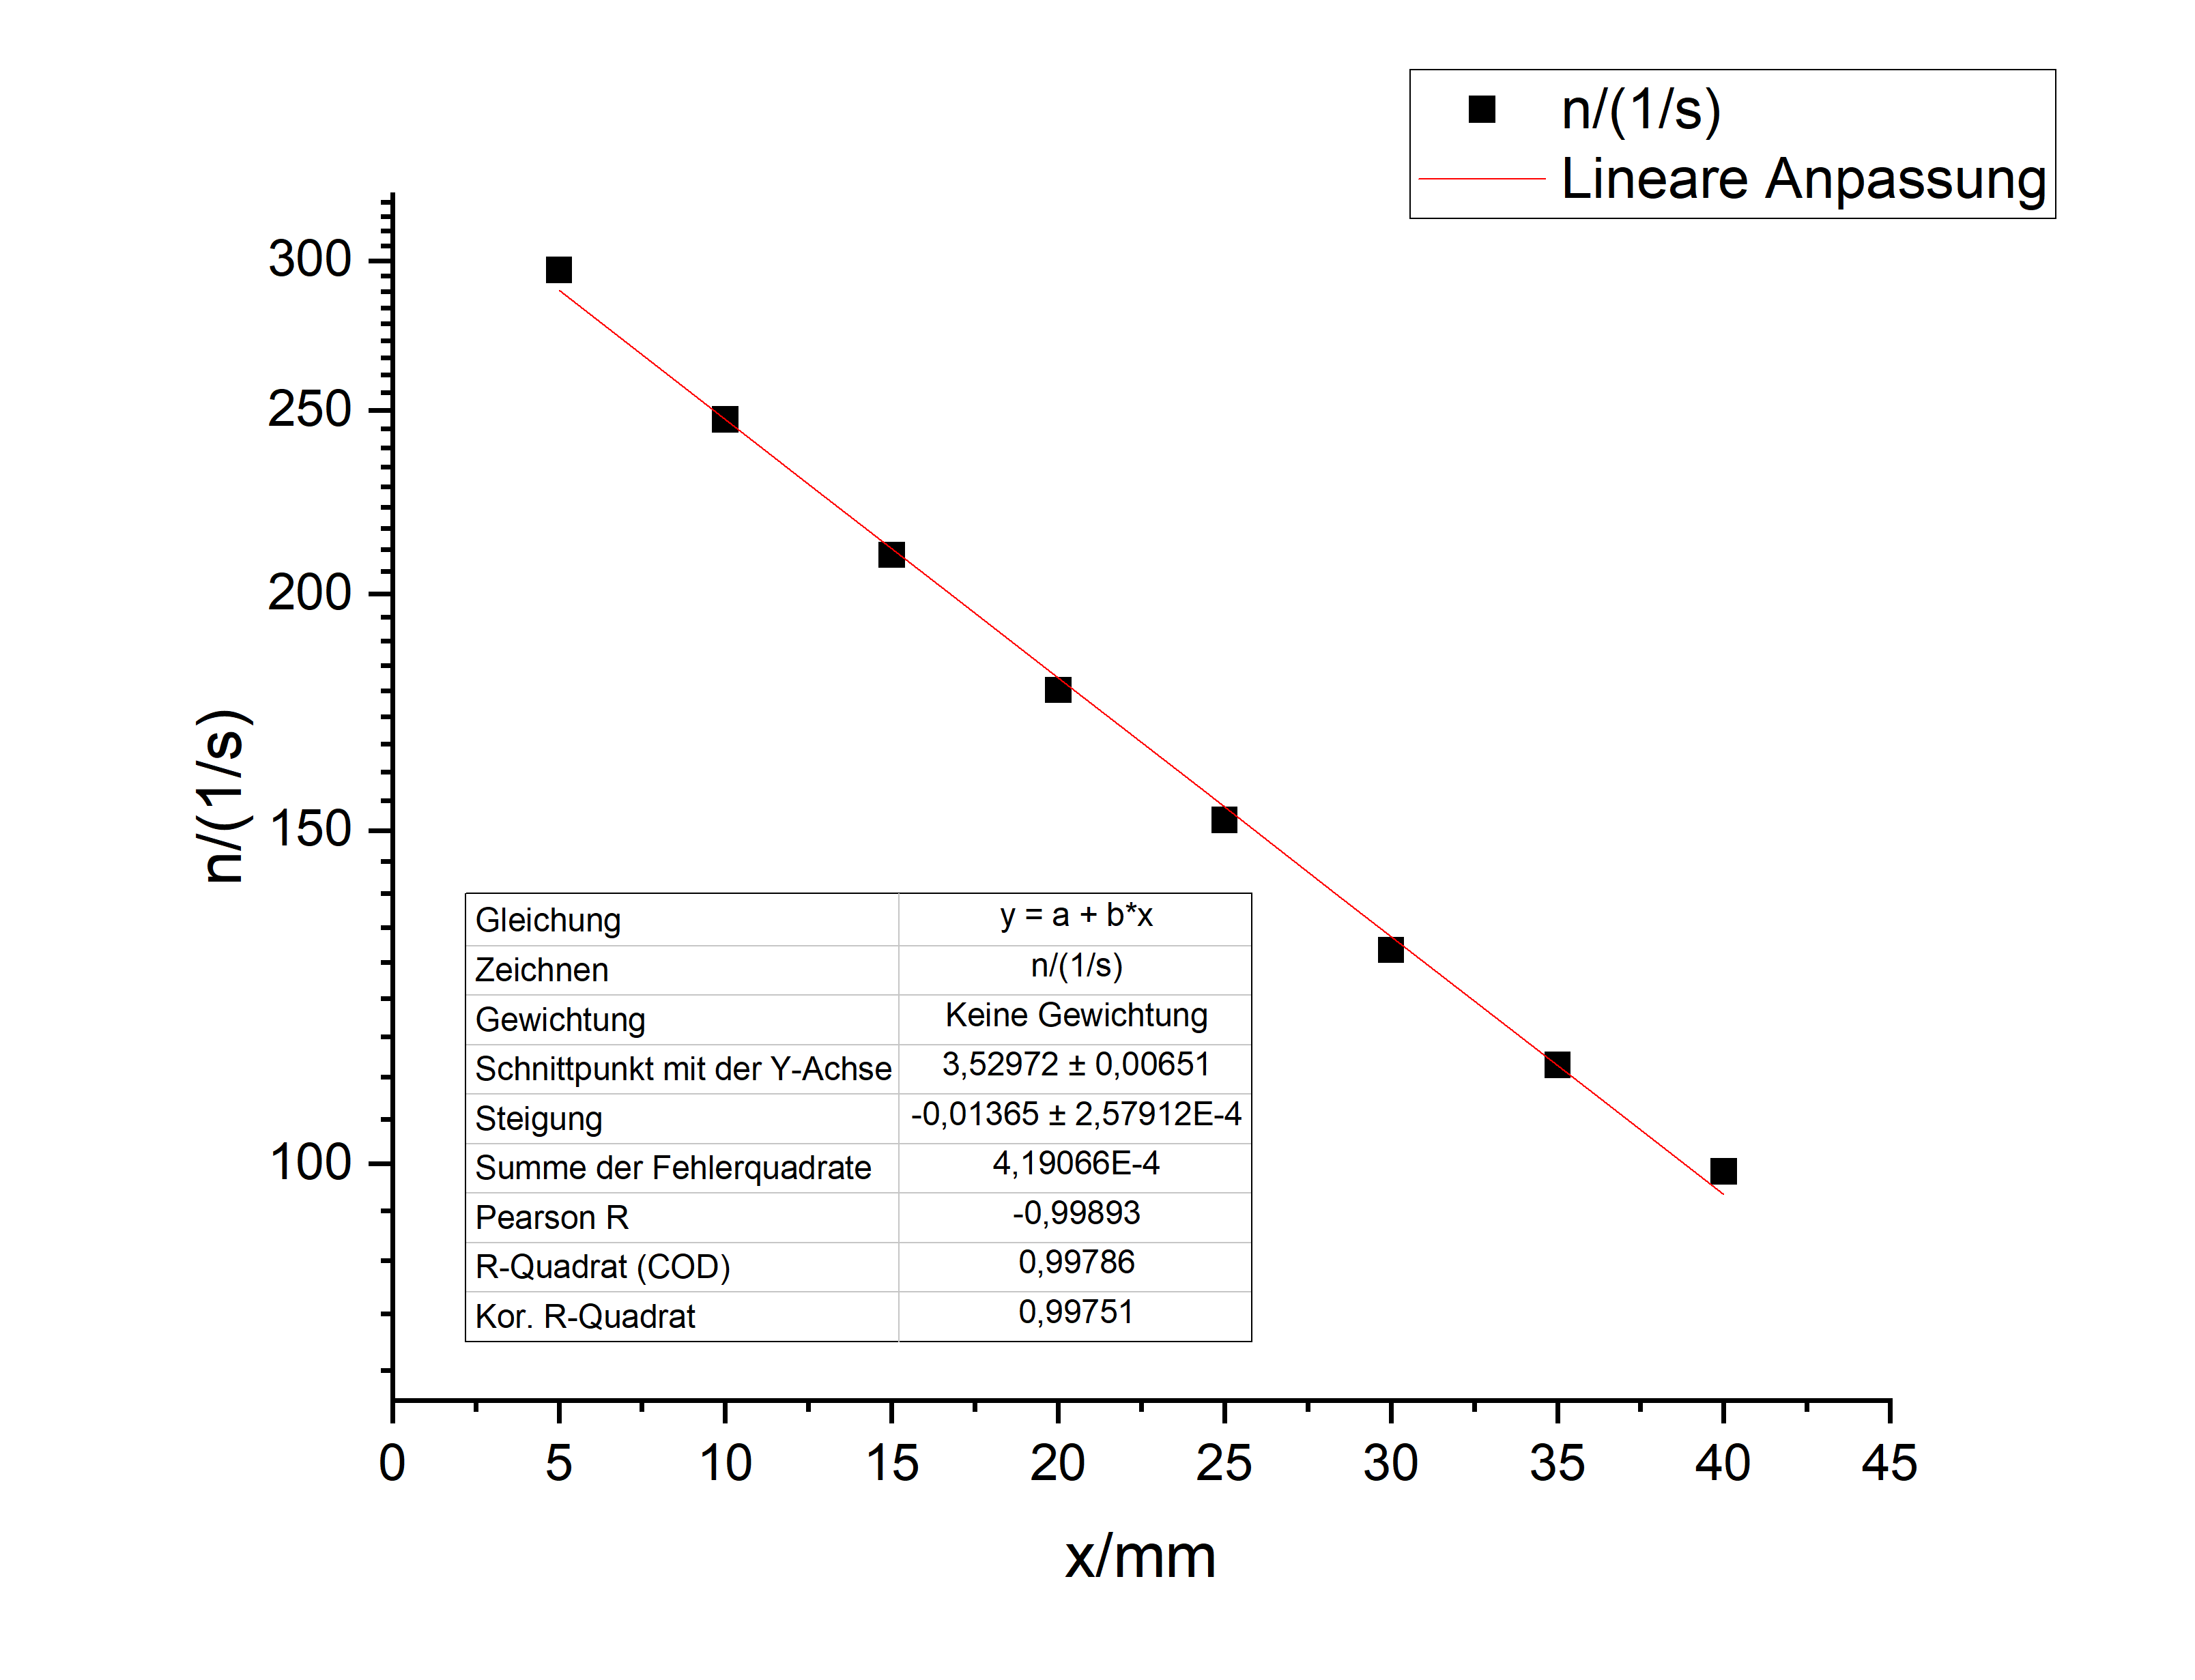
\includegraphics[width=0.8\textwidth]{2023-04-24 - V3 - Radioaktivität/images/versuch3/beta1.png}
    \caption{n über x halblogarithmisch aufgetragen}
    \label{beta1}
\end{figure}
Aus der Steigung des scheinbaren Fits der Funktion ergibt sich ein Abschwächungskoeffizient von Aluminium von $0,0136 \pm 2,5791 \cdot 10^{-4}$ $1/mm$.
\end{document}